%%%%%%%%%%%%%%%%%%%%%%%%%%%%%%%%%%%%%%%%%%%%%%%%%%%%%%%%%%%%%%%%%%%%%%%%%%%%%%%
%%                                                                       THEORY
%%%%%%%%%%%%%%%%%%%%%%%%%%%%%%%%%%%%%%%%%%%%%%%%%%%%%%%%%%%%%%%%%%%%%%%%%%%%%%%
%%                                          the standard modell and other stuff



%______________________________________________________________________________
%                                                     Theoretischer Hintergrund
\chapter{Theoretischer Hintergrund}

\begin{quote}
    The abstact comes last
\end{quote}



%______________________________________________________________________________
%                                                               Standard-Modell
\section{Das Standardmodell der Teilchenphysik}
\label{theory:standardmodell}

% + Einführung (Quarks, Leptonen, Wechselwirkungen, Eichinvarianz)
% + Starke Wechselwirkung (Farbladung, Confinement)
% + Elektroschwache Theorie (GSW, Mischungswinkel)
% + Spontane-Symmetriebrechung (Higgs-Mechanismus)

Das Standardmodell der Teilchenphysik beschreibt die Dynamik subatomarer
Teilchen auf der Basis von drei fundamentalen Wechselwirkungen, der
elektromagnetischen, der schwachen und der starken Wechselwirkung.
Außerordentlich erfolgreich in der Erklärung einer Vielzahl experimenteller
Resultate, wurde die Existenz mehrerer heute bekannter Teilchen bereits vor
deren Entdeckung vom Standardmodell vorhergesagt. Der erst kürzlich erfolgte
experimentelle Nachweis des Higgs-Bosons durch das ATLAS-Experiment
(\cite{Aad:2012tfa}) komplettiert die Liste der vom Standardmodell postulierten
Teilchen und führt dessen Erfolg fort.

Das Standardmodell unterscheidet zwei Klassen von Teilchen. Die Bosonen mit
ganzzahligem Spin, welche die Austauschteilchen der fundamentalen
Wechselwirkungen repräsentieren und die Fermionen mit halbzahligem Spin, die
die Bausteine der bekannten Materie sind und auschließlich über den Austauch
von Bosonen miteinander wechselwirken.  

Mathematisch beschrieben wird das Standardmodell durch Quantenfeldtheorien. Die
\ac{QED} erklärt dabei die elektromagnetische und die schwache Wechselwirkung,
während die \ac{QCD} die starke Wechselwirkung begründet. Beide sind
Eichtheorien, sodass die Forderung nach lokaler Eichinvarianz der
Lagrangedichten die Existenz der Austauschteilchen, den Eichbosonen, notwendig
macht. Es hängt dabei von der jeweiligen Symmetriegruppe ab, wie viele
Eichbosonen benötigt werden. Das bekannteste Eichboson ist das Photon
($\gamma$), welches die elektromagnetische Wechselwirkung vermittelt, selbst
aber ungeladen und masselos ist. Die schwache Wechselwirkung hingegen kennt
drei Austauschteilchen, die beiden geladenen $W^\pm$ Bosonen und das neutrale
Z-Boson. Alle drei besitzen eine nicht-verschwindende Masse, was nachträgliche
Einführung des Higgs-Mechanismus\footnote{siehe Abschnitt \ref{}}
notwendig gemacht hat. Die Bosonen der starken Wechselwirkung sind die acht
Gluonen ($g$), die wiederum masselos sind keine elektrische Ladung Tragen. Eine
Übersicht über die Austauschteilchen ist in Tabelle \ref{tab:bosons} zu finden.

\begin{table}
    \centering
    \begin{tabular}{|c|c|c|c|c|}
        \hline
        \bf{Eichboson} & \bf{Symbol} & \bf{Masse} $[\GeV]$ & \bf{Ladung} &
        \bf{Wechselwirkung} \\
        \hline\hline
        Photon        & $\gamma$ & $0$       & $0$        & elektromagnetisch \\
        $W^\pm$-Boson & $W^\pm$  & $80,385 $ & $\pm 1\;e$ & schwach \\
        $Z$-Boson     & $Z$      & $91,1876$ & $0$        & schwach \\
        Gluon         & $g$      & $0$       & $0$        & stark \\
        \hline
    \end{tabular}
    \caption[Die Eichbosonen des Standardmodells]
        {Die Eichbosonen des Standardmodells mit Massen
        (\cite{PhysRevD.86.010001}) und Ladung}
    \label{tab:bosons}
\end{table}

Die Fermionen werden unterschieden in solche mit ganzahliger elektrischer
Ladung, den Leptonen, und jene mit drittelzahliger Ladungen, den Quarks. Die
Familie der Leptonen umfasst drei geladene ($Q=-1e$) Teilchen, das Elektron
($e^-$), das Myon ($\mu^-$) und das Tauon ($\tau^-$) und jeweils dazuhörige
ungeladene Neutrinos ($\nu_e,\nu_\mu,\nu_\tau$). Die geladenen Leptonen
wechselwirken sowohl elektromagnetisch, als auch über die schwache
Wechselwirkung, während die elektrisch neutralen Neutrinos lediglich an der
schwachen Wechselwirkung beteiligt sind. Die Massen der geladenen Leptonen sind
wohl bekannt, während für die Massen der Neutrino bloß obere Grenzen angegeben
werden können. Deren absolute Werte und vor allem deren Hierarchie sind
Gegenstand aktueller Forschung\footnote{siehe zum Beispiel
\cite{Winter:2013ema}}. Unter den Quarks, den Konstituenten hadronischer
Materie, existieren solche mit Ladung $Q=+\tfrac{2}{3}e$, die sogenannten
\textit{up-type} Quarks, und solche mit $Q=-\tfrac{1}{3}e$, die
\textit{down-type} Quarks. Alle Quarks koppeln neben der elektromagnetischen
und schwachen Wechselwirkung, zudem noch über die starke Wechselwirkung.
Zu allen Fermionen existieren entsprechende Antiteilchen, die sich zu ihrem
jeweiligen Teilchenpartner nur durch deren Quantenzahlen unterscheiden. Tabelle
\ref{tab:fermions} listet die Fermionen des Standardmodells, wobei auf die
Aufführung der Antiteilchen der Einfachheit halber verzichtet wurde.

\begin{table}
    \centering
    \begin{tabular}{|l|c|l|c|}
        \hline
        \bf{Lepton} & \bf{Symbol} & \bf{Masse} & \bf{Ladung} \\
        \hline\hline
        Elektron          & $e^-$      & $0,511 \MeV$             & $-1\;e$ \\
        Elektron-Neutrino & $\nu_e$    & $<0,205 \eV$ (95\%C.L.)  & $0$     \\
        \hline
        Myon              & $\mu^-$    & $105,658 \MeV$           & $-1\;e$ \\
        Myon-Neutrino     & $\nu_\mu$  & $<0,19 \MeV$  (90\%C.L.) & $0$     \\
        \hline
        Tauon             & $\tau^-$   & $1776,82 \MeV$           & $-1\;e$ \\
        Tauon-Neutrino    & $\nu_\tau$ & $<18,2 \MeV$  (95\%C.L.) & $0$     \\
        \hline\hline
        \bf{Quark} & \bf{Symbol} & \bf{Masse} & \bf{Ladung} \\
        \hline\hline
        up      & $u$ & $2,3 \MeV$    & $+2/3\;e$ \\
        down    & $d$ & $4,8 \MeV$    & $-1/3\;e$ \\
        \hline
        charm   & $c$ & $1,275 \GeV$  & $+2/3\;e$ \\
        strange & $s$ & $95  \MeV$    & $-1/3\;e$ \\
        \hline
        top     & $t$ & $4,66 \GeV$   & $+2/3\;e$ \\
        bottom  & $b$ & $173,07 \GeV$ & $-1/3\;e$ \\
        \hline
    \end{tabular}
    \caption[Die Fermionen des Standardmodells]
        {Die Fermionen des Standardmodells mit Massen
        (\cite{PhysRevD.86.010001}) und Ladung}
    \label{tab:fermions}
\end{table}



\subsection{Phenomenologie der starken Wechselwirkung}
Die starke Wechselwirkung erklärt die Dynamik zwischen den Quarks und wird
mathematisch durch die $SU(3)$ symmetrische \ac{QCD} beschrieben. Die $SU(3)$
Gruppe wird durch 8 Generatoren erzeugt, deren physikalische Entsprechung die 8
Gluonen, der starken Wechselwirkung sind. Die hier relevante Quantenzahl ist
die sogenannte \textit{Farbladung}, welche die Ausprägungen rot, grün und blau
bzw. antirot, antigrün und antiblau annehmen kann, wobei die Summe aller drei
(Anti-)Farben Null ergibt - man spricht von einem \textit{weißen}
Zustand\footnote{In Analogie zur additiven Farbmischung}. Gluonen tragen stets
eine Farb- und eine Antifarbladung, während (Anti-)Quarks immer nur eine
(Anti-)Farbe tragen, die durch den Austausch entsprechender Gluonen geändert
werden kann. Für die Gluonen ergeben sich mathematisch aus dem direkten Produkt
des Farbtripletts mit dem Antifarbtriplett ein Farb-Oktett und ein
Farb-Singulatt, also 8+1 Zustände. Der Singulett-Zuständ wäre aber
total-symmetrisch und somit farbneutral, was in der Natur nicht beobachtet. Aus
diesem Grund verwirft man den Singulett-Zustand und ordnet die übrigen acht
Zustände den 8 Gluonen zu.

Ebenso beobachtet man keine freien farbneutralen Quarks, was man zum Phänomen
des \textit{Confinement} erklärt hat, welches besagt, dass Quarks sich stets
entweder zu Quark-Antiquark Paaren, sogenannten Mesonen, oder Kombinationen aus
drei (Anti-)Quarks, sogenannter Baryonen, zusammenschließen, um nach außen hin
die Farbneutralität zu gewährleisten. Die Menge von Mesonen und Baryonen fasst
man unter dem Begriff Hadronen zusammen, weshalb der eben beschriebene Prozess
der Bildung von Bindungszuständen von Quarks \textit{Hadronisierung} genannt
wird.

Die Auswirkungen des Confinement spiegeln sich auch in der Kopplungsstärke der
starken Wechselwirkung wieder, denn im Gegensatz zur elektromagnetischen Kraft,
bei der mit größer werdenden Abständen das Potential immer kleiner wird, wächst
die Kraft der starken Wechselwirkung mit größeren Abständen an. Die Ursache
liegt in der sog. Asymptotischen Freiheit, die in allen nicht-abelschen SU(3)
Theorien, wie der QCD auftritt und bewirkt, dass mit kleiner werdenden Energien
also größer werdenden Abständen der Betrag der Kopplungskonstanten steigt.



\subsection{Elektroschwache Theorie}
\label{theory:electroweak}
Die elektromagnetische und die schwache Wechselwirkung konnten von Salam,
Glashow und Weinberg erfolgreich in einer einzigen
\textit{elektroschwachen} Theorie vereinheitlicht werden, wofür sie 1979 mit
dem Physik-Nobelpreis ausgezeichnet wurden. Die mathematische Beschreibung
erfolgt durch die $SU(2)_L \times U(1)_Y$ Symmetrie-Gruppe.

Die $SU(2)_L$ repräsentiert dabei die schwache Wechselwirkung, die nur an
links-chirale Teilchen koppelt, worauf der Index $L$ hinweist. Die assoziierte
Quantenzahl ist der sogenannte \textit{schwache Isospin} $T$, nachdem die
wechselwirkenden Fermionen in Isospin-Dubletts ($T=\frac{1}{2})$ klassifiziert
werden können und innerhalb derer sich die Teilchen identisch bezüglich der
schwachen Wechselwirkung verhalten.
\begin{equation*}
    \left.
    \binom{\nu_e}{e^-}_L , \binom{\nu_\mu}{\mu^-}_L ,
    \binom{\nu_\tau}{\tau^-}_L
    \right|
    \binom{u}{d'}_L , \binom{c}{s'}_L , \binom{t}{b'}_L 
    \qquad\qquad
    \binom{T_3 = +\frac{1}{2}}{T_3 = -\frac{1}{2}}
\end{equation*}
Die entsprechenden Teilchen mit rechtshändiger Chiralität Tragen einen
schwachen Isospin von $T=0$ und nehmen nicht an der schwachen Wechselwirkung
teil, bzw. sind nicht existent, wie im Falle der rechts-chiraler Neutrinos. Die
Zustände $d',s',b'$ bezeichnen die down-type Quarkzustände der schwachen
Wechselwirkung, die über die CKM-Matrix\footnote{siehe zum Beispiel 
\cite{PhysRevD.86.010001}} mit den entsprechenden Zuständen der starken
Wechselwirkung verknüpft sind. Die Eichinvarianz der SU(2) impliziert das
Vorhandensein von drei Austauschboson, die hier mit $W^i\; (i=1,2,3)$
bezeichnet werden und zusammen ein Isospin-Triplett mit $T=1$ bilden. Die
$U(1)_Y$ Symmetrie-Gruppe führt ein weiteres Eichboson $B^0$ in die
elektroschwache Theorie ein, das mit der Quantenzahl der schwachen Hyperladung
$Y$ verknüpft ist. Diese beträgt für alle linkschiralen Leptonen $Y=-1$ und
alle linkschiralen Quarks $Y=-\frac{1}{3}$. Somit ist es möglich eine Beziehung
zwischen der schwachen Hyperladung, dem schwachen Isospin und der elektrischen
Ladung eines Leptons anzugeben:
\begin{equation}
    Q = T_3 + \frac{Y}{2}
    \label{eq:charge_relation}
\end{equation}

Die vier bisher vorgestellten Eichbosonen $W^i$ und $B^0$ haben keine Masse, da
jeder massenbehaftete Eichterm die Symmetrie der Langrangedichte zerstören
würde. Aus diesem Grund sind die $W^i$ und $B^0$ nicht mit den in Abschnitt
\ref{theory:standardmodell} eingeführten physikalisch beobachteten Bosonen
($W^\pm, Z, \gamma$) der elektromagnetischen und schwachen Wechselwirkung
identifizierbar, die abgesehen vom Photon in Realität massenbehaftet auftreten.
Der Effekt der spontanen Symmetriebrechung bewirkt, dass die physikalischen
Zustände als Rotation aus den masselosen Eichbosonen hervorgehen.
\begin{alignat*}{4}
    \gamma &\;=\;  &B^0 \cos\theta_W + W^3\sin\theta_W \\
    Z      &\;=\; -&B^0 \sin\theta_W + W^3\cos\theta_W
\end{alignat*}
Hierbei ist $\theta_W$ der nach S.Weinberg benannte Weinberg-Winkel, auch mit
\textit{schwacher Mischungswinkel} bezeichnet. Die $W^\pm$-Bosonen gehen aus den
masselosen $W^{1,2}$-Eichbosonen durch
\begin{equation*}
    W^\pm \;=\; \frac{1}{\sqrt{2}} \left( W^1 \mp W^2 \right)
\end{equation*}
hervor. Während die geladenen $W^\pm$-Bosonen aufgrund ihrerer Komposition aus
den nur an links-chirale Fermionen koppelnde $W^{1,2}$-Bosonen die Parität
maximal verletzen, bewirkt die Mischung mit dem $B^0$-Feld, dass die elektrisch
neutralen Photonen und $Z$-Bosonen auch an rechts-chirale Teilchen koppeln.

Bei der Berechnung von Matrixelementen mithilfe der Feynman-Regeln treten
für jeden Vertex Terme auf, die die oben beschriebenen Kopplungen
charakterisieren. Für den in dieser Arbeit interessanten Fall der Kopplung
eines Z-Bosons an zwei geladene Leptonen (siehe Abbildung
unten) findet man als Vertex-Faktor: \\
\begin{minipage}{0.6\textwidth}
\begin{equation}
    -i \frac{g\gamma^\mu}{\cos\theta_W} \left( \frac{1+\gamma^5}{2} c_R
        + \frac{1-\gamma^5}{2} c_L \right)
    \label{eq:coupling}
\end{equation}
\end{minipage}
\hfill
\begin{minipage}{0.3\textwidth}
    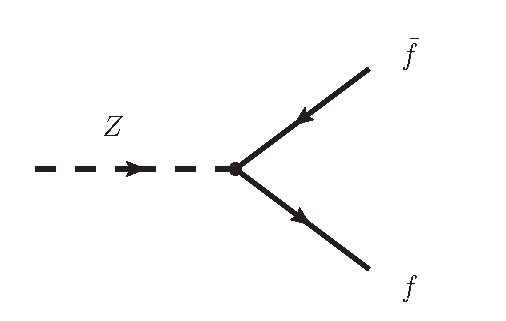
\includegraphics[width=1.0\textwidth]{img/NCvertex}
\end{minipage}
\newline

Hierbei ist $g$ die Kopplungskonstante, die ebenfalls über den Weinberg-Winkel
mit der Elementarladung zusammenhängt ($g\sin\theta_W=e$). Die $c_R$ bzw.
$c_L$ bezeichnen die Kopplungskonstanten für die rechts- bzw. links-chiralen
Anteile der Fermion-Felder, die durch die davorstehenden Operatoren\footnote{In
den Projektion-Operatoren $\frac{1+\gamma^5}{2}$ bzw. $\frac{1+\gamma^5}{2}$
taucht die $\gamma^5$ Matrix auf, die zu den Dirac'schen gamma-Matrizen gehört
und als $\gamma^5=i\gamma^0\gamma^1\gamma^2\gamma^3$ definiert ist.}
herausprojeziert werden. Für diese gilt:
\begin{align}
    c_L &= - \frac{1}{2} + \sin^2\theta_W   \\
    c_R &= \sin^2\theta_W
\end{align}
Alternativ lässt sich Gleichung (\ref{eq:coupling}) anstelle mit den links-
und rechts-chiralen Kopplungskonstanten auch mit Vektor- ($c_V=c_L+c_R$) und
Axialvektorkopplungen ($c_A=c_L-c_R$) schreiben:
\begin{equation}
    -i \frac{g\gamma^\mu}{\cos\theta_W} \left( \frac{c_V-c_A\gamma^5}{2}\right)
\end{equation}
Für die ungeladenen Leptonen und die Quarks lassen sich analoge
Kopplungskonstanten finden.
%, die in Tabelle \ref{tab:couplings} gelistet sind.
%\begin{table}
%    \centering
%    \renewcommand{\arraystretch}{1.4}
%    \begin{tabular}{|c|r|r|}
%        \hline
%        \bf{Fermion} & $\mathbf{c_V}$ & $\mathbf{c_A}$ \\
%        \hline \hline
%        $\nu_e,\nu_\mu,\nu_\tau$ & $\frac{1}{2}$ & $\frac{1}{2}$ \\
%        $e^-,\mu^-,\tau^-$ & $-\frac{1}{2}+2\sin^2\theta_W$ & $-\frac{1}{2}$   \\
%        $u,c,t$ & $\frac{1}{2}-\frac{4}{3}\sin^2\theta_W$ & $\frac{1}{2}$   \\
%        $d,s,b$ & $-\frac{1}{2}+\frac{2}{3}\sin^2\theta_W$ & $-\frac{1}{2}$ \\
%        \hline
%    \end{tabular}
%    \caption{Vektor- und Axialvektorkopplungen der Fermionen an den neutralen
%        Strom}
%    \label{tab:couplings}
%\end{table}

Aufgrund der Renormalisierung der elektroschwachen Quantenfeldtheorie hängt der
Wert des schwachen Mischungswinkels $\theta_W$, oder in gebräuchlicherer
Notation $\sin^2\theta_W$, schwach von der betrachteten Energieskala $Q^2$
ab\footnote{Wegen der Relevanz für die vorliegende Arbeit beziehen sich alle
folgenden Bezüge oder Angaben zu $\sin^2\theta_W$ auf den Mischungswinkel am
Z-Pol ($Q^2=91,2\GeV$)}. Zudem werden bei der Renormalisierung einige
Korrekturterme höherer Ordnung absorbiert, während andere an Bedeutung
gewinnen. Deshalb wird für gewöhnlich ein effektiver Mischungwinkel definiert,
der gegenüber dem oben definierten Ausdruck verschoben ist:
\begin{equation}
    \sin^2\theta_W^\text{eff} = \sin^2\theta_W + 0,00029
    \label{eq:effective_angle}
\end{equation}
Der aktuell genauest bekannte Wert (\cite{PhysRevD.86.010001}) für den
effektiven schwachen Mischungswinkel beträgt:
\begin{equation}
    \sin^2\theta_W^\text{eff} = 0,23146 \pm 0,00012
    \label{eq:literature_value}
\end{equation}



\subsection{Spontane Symmetrie-Brechung und Higgs-Mechanismus}
Der Higgs-Mechanismus benutzt das Konzept der spontanen Symmetrie-Brechung, um
die Eichinvarianz und Renormierbarkeit der elektroschwachen Theorie
wiederherzustellen. Der scheinbare Widerspruch zwischen den masselos
statuierten Eichbosonen der $SU(2)_L \times U(1)_Y$ und den experimentell
beobachteten massiven $W^\pm$- und $Z$-Bosonen wird durch deren Wechselwirkung
mit einem den Raum durchziehenden Higgs-Feld behoben.

Der Higgs-Mechanismus führt in die Lagrange-Dichte der elektroschwachen Theorie
einen weiteren Term ein, dessen physikalische Entsprechung ein imaginäres
skalares Feld $\phi$ ist, das einem $SU(2)_L$ Dublett genügt.
\begin{equation}
    \phi = \binom{\phi^+}{\phi^0}
\end{equation}
Die Indizes $^+$ und $^0$ an den imaginär skalaren Komponenten des Feldes
deuten auf die resultierende elektrische Ladung hin\footnote{siehe Gleichung
\ref{eq:charge_relation} für $Y(\phi)=1$ und $T_3(\phi)=\pm\tfrac{1}{2}$}.
Der zusätzliche Term dieses Feldes in der Lagrange-Dichte ist
\begin{equation}
    \mathcal{L}_\text{Higgs} = (D_\mu\phi)^\dagger(D^\mu\phi) - V(\phi)
\end{equation}
mit dem Potential
\begin{equation}
    V(\phi) = \mu^2\phi^\dagger\phi + \lambda (\phi^\dagger\phi )^2
\end{equation}
Für $\mu^2<0$ folgt aus der Form des Potentials, dass der Vakuumerwartungswert
(Grundzustand), nicht mit dem Symmetriepunkt im Ursprung zusammenfällt, sondern
in der Form eines Kreises entartet ist:
\begin{equation}
    \braket{0\:|\phi|\:0} = \sqrt{\frac{-\mu^2}{\lambda}} \equiv \nu 
\end{equation}
Die spezielle Wahl des Grundzustandes $\braket{\phi_0}=\binom{0}{\nu/\sqrt{2}}$
hat nun zur Folge, dass die Symmetrie gebrochen gebrochen wird und den vier
Freiheitsgraden des Feldes $\phi$ nach dem Goldstone-Theorem vier skalare
Bosonen entsprechen müssen\footnote{Diese explizite Wahl stellt sicher, dass
das der Vakuumerwartungswert ungeldaden und reel ist}.

Führt man nun eine Entwicklung um diesen Punkt durch, so verbleibt lediglich
ein Freiheitsgrad, während die anderen drei von den Eichbosonen der $SU(2)_L$
\textit{absorbiert} werden und so deren Masse erzeugen. Der übrige
Freiheitsgrad ist nun in transversaler Richtung anregbar und entspricht somit
einem physikalischen massiven skalaren Boson, dem Higgs-Boson H(x).
\begin{equation}
    \phi(x) = \frac{1}{\sqrt{2}}\binom{0}{\nu+H(x)}
\end{equation}
Neben den Boson-Massen erzeugt das Higgs-Feld über Yukawa-Kopplungen auch die
Massen der Fermionen, obgleich deren Wert durch den Higgs-Mechanismus nicht
vorhergesagt wird. Dasselbe gilt auch für die Masse des Higgs-Bosons selbst,
die experimentell zu ermitteln bleibt.



%______________________________________________________________________________
%                                                               Hadron-Collider
\section{Physik mit Hadron-Collidern}
\label{theory:hadron_collider}

% + Luminosität, Schwerpunktsenergie}
% + PDFs

Mit Hadron-Collidern, wie dem \ac{LHC}, ist es möglich geladene Hadronen in
gegenläufigen Strahlen auf annähernd Lichtgeschwindigkeit zu beschleunigen und
diese an fest definierten Punkten zur Kollision zu bringen. Die experimentell
interessantesten Größen sind die Schwerpunktsenergie $\sqrt{s}$ und die
instantane Luminosität $L$. Letztere stellt einen Zusammenhang zwischen der
erwarteten Ereignisrate $\dot N$ und dem Wirkungsquerschnitt $\sigma_P$ des
betrachteten Prozesses dar.
\begin{equation}
    \dot N \;=\; L \cdot \sigma_P
\end{equation}
Die Teilchen laufen in Collidern in der Regel in Paketen, sogenannten
\textit{bunches} (vom engl. \textit{bunch}, Bündel), mit festdefiniertem
zeitlichen Abstand um. Die instantane Luminosität ergibt sich dann aus
\begin{equation}
    L = \frac{n N_1 N_2 f}{A}
\end{equation}
wobei $n$ die Anzahl der Bunches und $f$ die Frequenz deren Zusammentreffens
ist. $N_{1,2}$ bezeichnet die Anzahl der Teilchen pro Bunch, während $A$ die
Querschnittsfläche der Pakete ist. Damit hat die Luminostität die Einheit
$\centi\meter^{-2}\second^{-1}$.

Der Wirkungsquerschnitt $\sigma_P$ ist ein Maß für die Wahrscheinlichkeit einen
bestimmen Prozess zu beobachten und ist dabei von der zur Verfügung stehenden
Energie abhängig. Die kollidierenden Hadronen sind zusammengesetzte Teilchen,
sodass ab einer bestimmten Schwelle die Energien der Konstituenten die
eigentlich relevante Größe sind. Aufgrund der Relevanz für die vorliegende
Arbeit wird im folgenden von kollidierenden Protonen ausgegangen, deren Energie
sehr viel höher ist, als das elastische Streuprozesse relevant würden. Diese
sind aus drei Valenzquarks in der Kombination $uud$ und einem See aus
Quark-Antiquark Paaren und Gluonen aufgebaut. Die einzelnen Konstituenten
werden unter dem Begriff Partonen zusammengefasst, ein von Feynman und Bjorken
eingeführter Begriff und die Grundlage des sogenannten Partonmodells
(\cite{Bjorken:1968dy}). Man betrachtet dabei das Proton in einem Bezugssystem
in dem die Transversalimpulse und Ruhemassen der Partonen vernachlässigbar
sind\footnote{Dies ist im Falle von Hadron-Collidern, insbesondere des
\ac{LHC}, sehr gut erfüllt}. Dann lässt sich der Impuls eines Partons mit $x$
relativ zum Gesamtimpuls des Protons beschreiben

Innerhalb des Partonmodells lässt sich die Wahrscheinlichkeit ein Parton mit
einem Impulsbruchteil $x$ zu finden mit einer sogenannten \ac{PDF} beschreiben.
Dabei besteht generell eine zusätzliche Abhängigkeit zur betrachteten Skala
$Q^2$, da mit dieser die \textit{Auflösung} determiniert ist, mit der
Substrukturen in Hadronen analysiert werden können. In Proton-Proton
Kollisionen lässt sich der Wrikungsquerschnitt einer belieben Reaktion nun über
das Integral der \ac{PDF}s und das entprechende Matrixelement $M$ auf
Parton-Level ausdrücken:
\begin{equation}
    \sigma(pp\rightarrow X) \;=\; \sum_{a,b} \int_0^1 dx_a \int_0^1 dx_b \;
        f_a(x_a,Q^2) \: f_b(x_b,Q^2) \: M(s,x_a,x_b)
\end{equation}
Hierbei bezeichnet $s$ die verfügbare Schwerpunktsenergie im Proton-Proton
System und $f_a(x_a,Q^2)$ bzw. $f_b(x_b,Q^2)$ die \ac{PDF}s für die Partonen
$a$ und $b$.

Die \ac{PDF}s repräsentieren also das beste Wissen über den Aufbau und die
Dynamik innerhalb der Hadronen, müssen jedoch rein durch experiementelle Daten
bestimmt werden. Dazu verwendet man in großen Bereichen von $Q^2$ und $x$ die
gemessenen Wirkungsquerschnitte bekannter Prozesse und kombiniert die Daten
vieler Experimente. Abbildung \ref{fig:mstw} zeigt beispielhaft resultierende
\ac{PDF}s bei zwei verschiedenen Skalen $Q^2$.

\begin{figure}
    \centering
    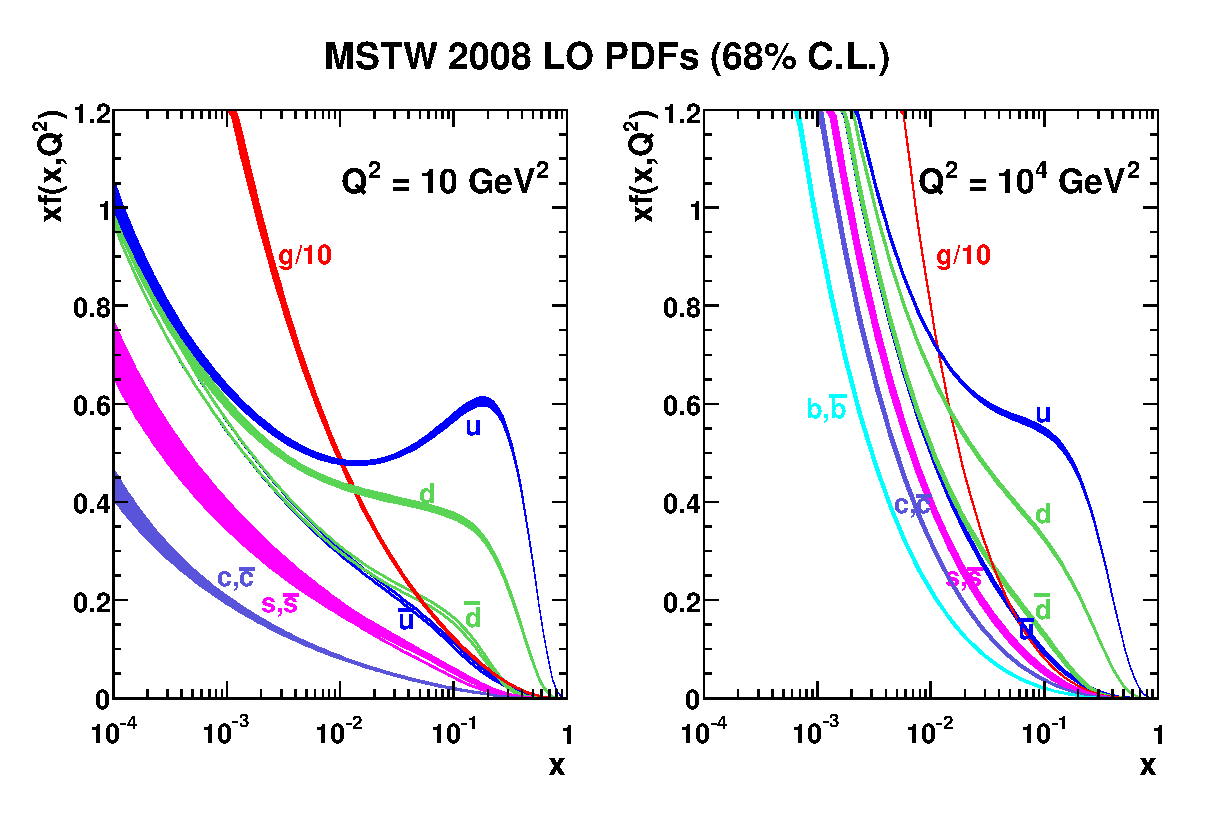
\includegraphics[width=0.8\textwidth]{img/mstw}
    \caption[Parton-Verteilungs-Funktionen bei $Q^2=100\GeV^2$ und
        $Q^2=10^4\GeV^2$]
        {Parton-Verteilungs-Funktionen bei \mbox{$Q^2=100\GeV^2$} und 
        \mbox{$Q^2=10^4\GeV^2$} bestimmt durch Martin, Stirling, Thorne und
        Watt \cite{Martin:2009iq}}
    \label{fig:mstw}
\end{figure}

Wie gut zu sehen ist haben die Verteilungsfunktionen für $u$- und $d$-Quarks
ein lokales Maximum bei großen $x$, was auf die Valenzquark Zusammensetzung des
Protons ($uud$) zurückzuführen ist. Die Verteilungen der übrigen Seequarks
sinkt erwartungsgemäß mit den größer werdenden Massen ab.  Außerdem zeigt sich
hier, dass die Seequark-Verteilungen für Quark und Antiquark identisch sind,
wodurch die elektrische Nettoladung des Protons von $1$ nach außen hin
sichergestellt ist. Beim Vergleich zwischen hohen und niedrigem $Q^2$ sieht
man, dass im letztgenannten Fall die Wahrscheinlichkeiten für Seequarks und
größer sind, als im Fall niedrieder Energie, was ebenfalls der Erwartung
entspricht.




%______________________________________________________________________________
%                                                 Vorwärts-Rückwärts Asymmetrie
\section{Vorwärts-Rückwärts Asymmetrie}
\label{theory:afb}

\begin{itemize}
    \item Theoretische Beschreibung
    \item Collins-Soper
    \item vorangegangene Messungen / andere Messmethoden
    \item Grund der Messung (Higgs-Constraints)
\end{itemize}



